% -*-coding: utf-8;-*-
% $Id: Part4.tex,v 1.9 2005-02-10 20:58:08 evlad Exp $
%%%%%%%%%%%%%%%%%%%%%%%%%%%%%%%%%%%%%%%%%%%%%%%%%%%%%%%%%%%%%%%%%
% Глава 4 - Управление мобильным роботом
%%%%%%%%%%%%%%%%%%%%%%%%%%%%%%%%%%%%%%%%%%%%%%%%%%%%%%%%%%%%%%%%%

Одной из актуальных задач теории автоматического регулирования
является управление движущимимся объектами.  Распространенным частным
случаем такого объекта является мобильный робот --- колесная тележка с
автономным управлением.  Количество специализаций мобильных роботов
невероятно велико: от транспортных тележек на автоматизированном
производстве до военных роботов--разведчиков и движущихся
исследовательских аппаратов на других планетах.

При всем многообразии разноуровневых задач, связанных с управлением
движением мобильного робота, всегда имеет место одна базовая ---
движение к неподвижной цели -- маяку --- по кратчайшей траектории.
При этом важна точность попадания в цель, поскольку она определяет
точность всех перемещений робота.  В зависимости от оснащенности
сенсорными и навигационными системами эта задача может решаться
по-разному.  Рассмотрим случай наличия единственного сенсора ---
видеокамеры с детектором положения маяка в поле её видимости.

\section{Описание робота}

Мобильный робот представляет собой тележку с тремя колесами, два из
которых расположены спереди и одно рояльное сзади.  Основные узлы
робота представлены на~\figref{fig:moby_projections}.  Передние колеса
являются ведущими и имеют независимые приводы $3$ и $4$.  Заднее
колесо расположено по средней оси платформы и не управляется.  Робот
оснащен системой технического зрения на основе видеокамеры $6$ с
инфракрасным фильтром.  Видеокамера закреплена неподвижно на
вертикальной мачте $7$.  На платформе также смонтированы компактный
компьютер $1$, система управления приводами $2$ и блок питания $5$.
Мобильный робот разработан сотрудниками и студентами кафедры
``Робототехнические системы и комплексы'' (РК-10)
МГТУ~им.~Н.~Э.~Баумана.

\begin{figure}[h]
\centerline{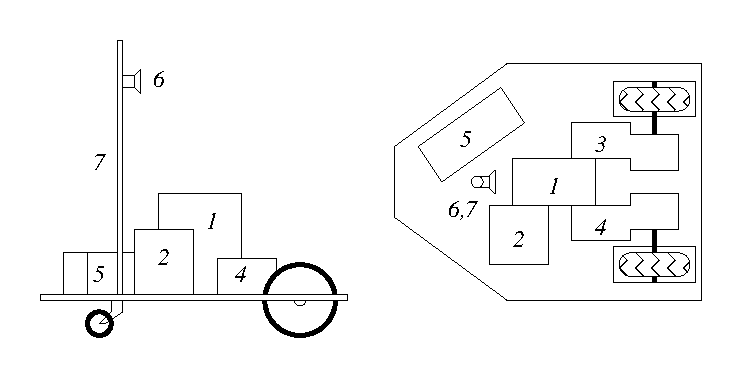
\includegraphics[width=0.8\textwidth]{moby_projections}}
\caption{Схема основных узлов мобильного робота (виды справа и сверху)}%
\label{fig:moby_projections}
\end{figure}

Каждый привод представляет собой двигатель постоянного тока, вал
которого связан с колесом через редуктор.  Известно, что
характеристики двигателей не идентичны.  В частности, одинаковое
напряжение, подаваемое на оба двигателя, приводит к разным скоростям
вращения валов.  Управление двигателями приводов осуществляется с
компьютера через блок $2$, преобразующим код широтно-импульсной
модуляции (ШИМ) в напряжение, подаваемое на двигатель.

Видеокамера является единственным сенсорным устройством мобильного
робота.  Изображение с камеры подается в компьютер робота через
специальный модуль, обеспечивающий оцифровку изображения.  Компьютер
мобильного робота PC-104 оснащен процессором Intel 80486, имеет
промышленное исполнение и архитектуру типового ПК.  Компьютер может
управляться как непосредственно, при присоединении клавиатуры и
монитора к блоку $1$, так и удаленно через локальную сеть, поскольку
робот оснащен сетевой картой Ethernet.

Компьютер робота находится под управлением операционной системы QNX,
обеспечивающей параллельное выполнение задач в режиме реального
времени.  Операционная система поддерживает удаленное управление со
стационарного ПК по сети.  Для QNX имеются компиляторы языков высокого
уровня, в том числе {\sf C} и {\sf C++}, что позволяет удобно
реализовывать произвольные алгоритмы управления.

Управление роботом производится в дискретном времени, причем шаг
квантования времени определяется быстродействием управляющего
компьютера, выполняющего служебные процессы ОС QNX, а также прикладные
программы: процесс оцифровки изображения с видеокамеры с получением на
выходе координат маяка и процесс управления приводами на основе
полученных координат.  Протоколирование времени показывает, что один и
тот же фрагмент кода в циклической части программы управления
приводами исполняется на процессоре каждые 0.25~с.  Этот шаг
квантования соблюдается достаточно точно несмотря на устаревший
процессор и параллельное выполнение нескольких процессов, что
свидетельствует о хорошем качестве QNX как ОС реального времени.

\section{Задача движения на маяк}

Рассмотрим задачу управляемого движения робота на неподвижный маяк,
находящийся в поле зрения видеокамеры.  В качестве маяка выступает
висящая лампа накаливания, хорошо заметная в инфракрасных лучах.  Цель
робота --- за кратчайшее время оказаться как можно ближе к маяку.  Эта
задача является одной из типовых на ежегодном молодежном
научно-техническом фестивале ``Мобильный робот''.

Будем считать, что в первый же момент времени только один маяк
находится в поле зрения видеокамеры и по мере движения робота другие
маяки в поле зрения не попадают.  Таким образом, не будем
рассматривать алгоритмы поиска маяка и отождествления целевого маяка
среди нескольких.

Координаты маяка в системе координат мобильного робота и даже
расстояние до него неизвестны.  Робот ``видит'' маяк только
посредством видеокамеры, то есть, известно угловое отклонение робота
от направления на маяк.  Данной информации недостаточно для расчета
оптимальной траектории, по которой робот достигнет цели.  В этих
условиях единственно возможным является управление по отклонению от
направления на маяк.  Входом объекта управления в этом случае
выступает напряжение на приводах, а наблюдаемым выходом ---
горизонтальная координата маяка (с нулем в центре поля зрения
видеокамеры).

Первоначально управление мобильным роботом осуществлялось программным
П-ре\-гу\-ля\-то\-ром с коэффициентом, подобранным эмпирическим путем.
Более сложные законы управления (ПИ, ПД, ПИД) не были реализованы в
силу трудоемкости оптимизации их параметров эмпирически.  В то же
время, аналитические методы для синтеза оптимального регулятора также
не применялись из-за трудности идентификации параметров объекта
управления.  Кроме того, достоверно известно о нелинейности ряда
компонентов системы.

Качество управления с помощью П-регулятора оказалось недостаточным при
повышении требований к точности ``попадания''.  Задача повышения
точности управляющего алгоритма особенно остро встала в связи с
управлением движением робота по сложному маршруту, когда видимый маяк
подменяется фиктивным, ``двигающимся'' по целевой траектории впереди
мобильного робота.

Поскольку алгоритм управления по условию задачи не имеет информации о
приближении к маяку, цель управления --- минимизация ошибки
``попадания'' в маяк --- становится эквивалентной задаче минимизации
отклонения робота от направления на маяк по всей траектории движения.
Данная задача с учетом наличия удовлетворительно функционирующего
П-регулятора подходит для решения с помощью методики синтеза
стохастического нейросетевого оптимального регулятора, описанной
в главах~\ref{linear_to_neural} и~\ref{neural_optimal_control}.

\subsection{Управление приводами}

Как уже отмечалось, робот оснащен двумя приводами ведущих колес,
независимо управляемыми с компьютера.  Для упрощения задачи будем
считать, что вместо двух каналов воздействия на объект (приводов)
имеется только один --- разница между напряжениями, подаваемыми на
приводы $\Delta u$.  Назовем его {\it управляющим дифференциалом}.
$$\begin{array}{l}
u_L=u_0-\Delta u\\
u_R=u_0+\Delta u
\end{array}$$

Для обеспечения поступательного движения робота задается постоянное
значение напряжения $u_0$, подаваемого на приводы.  Для поворота
робота направо следует задать $\Delta u<0$.  В этом случае левое
колесо будет вращаться быстрее правого и робот будет поворачиваться
вправо.

\subsection{Локация маяка}

Поскольку робот перемещается в горизонтальной плоскости, нас будет
интересовать горизонтальная координата маяка в поле зрения
видеокамеры, принцип формирования которой в зависимости от положения
маяка иллюстрируется на \figref{fig:moby_eye_coord}.
\begin{figure}
\centerline{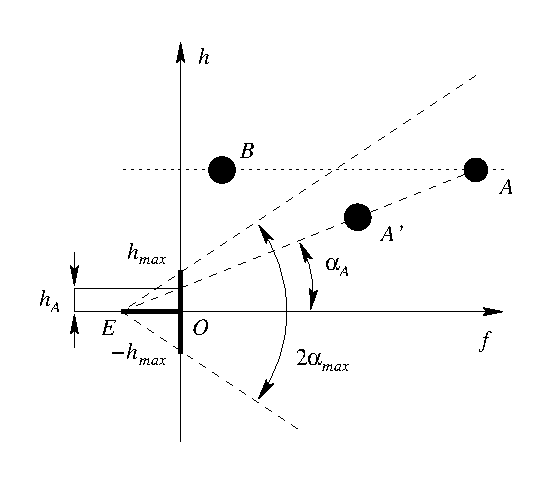
\includegraphics{moby_eye_coord_h}}
\caption{Координаты маяка в поле зрения видеокамеры мобильного робота
         (вид сверху)}
\label{fig:moby_eye_coord}
\end{figure}

Точка $E$ на схеме является воображаемым центром, в который сходятся
лучи из маяков.  Ось $f$ проходит через видеокамеру и совпадает с
направлением прямолинейного движения робота в текущий момент времени.
В силу ограниченности поля зрения видеокамеры углом $2\alpha_{max}$
маяки, расположенные в точках $A$ и $A'$, видны, а в точке $B$ --- нет.
На пути лучей имеется экран (поле зрения видеокамеры) с центром в
точке $O$.  Точка пересечения луча от маяка $A$ с экраном дает
координату $h_A$, поступающую из видеокамеры в компьютер.  Как угловая
координата $\alpha$ ограничена в диапазоне $[-\alpha_{max},
\alpha_{max}]$, так и отметка маяка на экране ограничена в диапазоне
$[-h_{max}, h_{max}]$.

Информация, поступающая в компьютер от видеокамеры, равномерно
дискретизирована от $-N\Delta h$ до $N\Delta h$, где $\Delta h$ ---
шаг дискретизации координаты маяка, а $2N+1$ --- число дискретных
точек на экране видеокамеры.  Очевидно, что равномерная дискретизация
экранных координат $h$ соответствует неравномерной дискретизации
угловой координаты $\alpha$ из-за тригонометрической связи между этими
параметрами.  Это одно из проявлений нелинейности объекта управления.
Кроме того, по мере приближения к неподвижному маяку чувствительность
координаты к управляющему воздействию существенно возрастает: малейшее
изменение управляющего дифференциала приводит в конце траектории к
большому изменению координаты маяка.

По схеме видно, что угловые координаты маяков, расположенных в точках
$A$ и $A'$ совпадают при том, что расстояние до них разное.  Однако
видеокамера не в состоянии распознать различие.

Пример траектории движения мобильного робота на маяк в горизонтальной
плоскости $xy$ приводится на \figref{fig:moby_trajectory}а.
\begin{figure}
\centerline{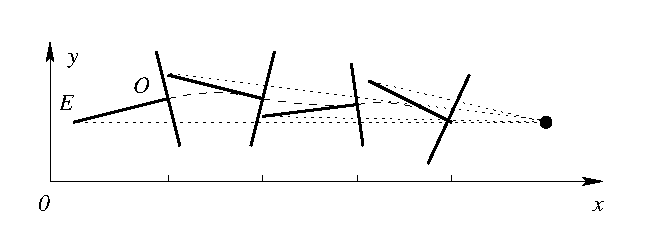
\includegraphics{moby_trajectory_a}}
\centerline{а)}
\centerline{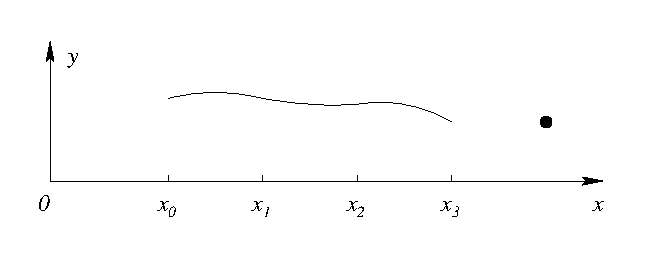
\includegraphics{moby_trajectory_b}}
\centerline{б)}
\centerline{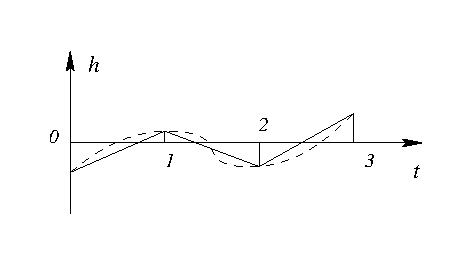
\includegraphics{moby_trajectory_c}}
\centerline{в)}
\caption{Траектория движения мобильного робота с промежуточными положениями
         платформы (а) и без них (б), а также траектория маяка в поле зрения
         видеокамеры (в)}
\label{fig:moby_trajectory}
\end{figure}

Объект управления, таким образом, можно представить в виде функции
управляющего дифференциала $\Delta u_k$ и некоторого внутреннего
состояния $\mathbf{s}$.  Выходом объекта управления является $h_{k+1}$
--- экранная координата маяка в поле зрения видеокамеры.
\begin{equation}\label{eq:mobot-function}
h_{k+1}=g(\Delta u_k, \mathbf{s})
\end{equation}

\section{Синтез нейросетевого регулятора}

Как уже отмечалось, оптимизация движения на маяк по угловому
отклонению без знания расстояния до маяка эквивалентна задаче
минимизации отклонения по траектории.  Учитывая это, можно применить
методику построения нейросетевого оптимального регулятора, изложенную
в предыдущих главах.  Поскольку ставится задача попадания в маяк,
уставка равна нулю и среднеквадратичный критерий
оптимизации~\eqref{eq:noc_synthesis_task} принимает вид:
\begin{equation}\label{eq:mobot-task}
  \sum\limits_k\big(g(u_k,\mathbf{s})-n_k\big)^2\rightarrow\min
\end{equation}

По методике для построения НОР необходимо решить следующие подзадачи:
\begin{enumerate}
\item Выбрать количество и номенклатуру входов НС--Р и НС--О, а также
      задать их внутренную структуру.

\item Собрать необходимые данные для обучения НС--Р имитации имеющегося
      П-регулятора и обучить его вне контура управления.

\item Собрать необходимые данные для обучения нейросетевой модели
      объекта управления и обучить её вне контура управления.

\item Заменить П-регулятор на нейросетевой и обучать его в контуре
      управления с помощью нейросетевой модели.
\end{enumerate}

Для проверки функционирования нейросетевого регулятора при управлении
мобильным роботом и сравнения точности управления с исходным линейным
регулятором был проведен натурный эксперимент.  Сравнение точности
``попадания'' в маяк осуществлялось измерением минимального расстояния
от траектории робота до прекции маяка на горизонтальную плоскость.
Траекторией движения робота было решено считать след точки,
находящейся на передней кромке платформы по оси симметрии.  В этой
точке находился закрепленный карандаш, оставлявший след на листе
бумаги, расположенном под маяком.

Погрешность определения точки проекции маяка на лист бумаги составляет
5 мм (радиус груза отвеса).  Погрешность рисования траектории равна 1
мм (толщина грифеля карандаша).  Погрешность измерения минимального
расстояния от траектории до проекции маяка составляет 2 мм.

\subsection{Архитектура и обучение нейросетевого регулятора}

Опираясь на рекомендации, сформулированные в п.~\ref{nnc_inputs}, в
случае нулевой уставки нецелесообразно использовать в качестве входов
пару $r_k,e_k$, поскольку уставка равна нулю.  Возьмем в качестве
входов $e_k,\Delta e_k$.  Это позволяет напрямую передать в НС--Р
информацию об ошибке и её первой производной.

Учитывая, что управлять придется реальным нелинейным объектом,
рационально взять нейросеть с достаточно сложной архитектурой: с двумя
скрытыми слоями с 5 и 3 нейронами в них.  В итоге имеем архитектуру
НС--Р $\NN^p_{2,5,3,1}(e_k,\Delta e_k)$.

Сбор данных для обучения осуществлялся путем протоколирования
управляющего дифференциала и координаты маяка в поле видеокамеры в
процессе десяти заездов с исходным П-регулятором.  Собранные данные
${e_k,u_k}$ были разделены на обучающие и тестовые.  Пакетное обучение
проходило с коэффициентом $\eta=0.01$ для скрытых слоев и $\eta=0.001$
для выходного нейрона.  По истечении 653 эпох было обнаружено
постепенное увеличение ошибки имитации на тестовой выборке и процесс
обучения был завершен.

Траектория ошибки воспроизведения по обучающей и тестовой выборкам в
процессе пакетного обучения приведены
на~\figref{fig:moby_nnc_pretr_training}.  Примеры траекторий,
использовавшихся для обучения и результат их имитации приведены
на~\figref{fig:moby_nnc_pretr}.

\begin{figure}
\centering
  \begin{tabular}{rc}
    \begin{sideways}
      {\hspace{4cm}\small Ошибка}
    \end{sideways}
    &
    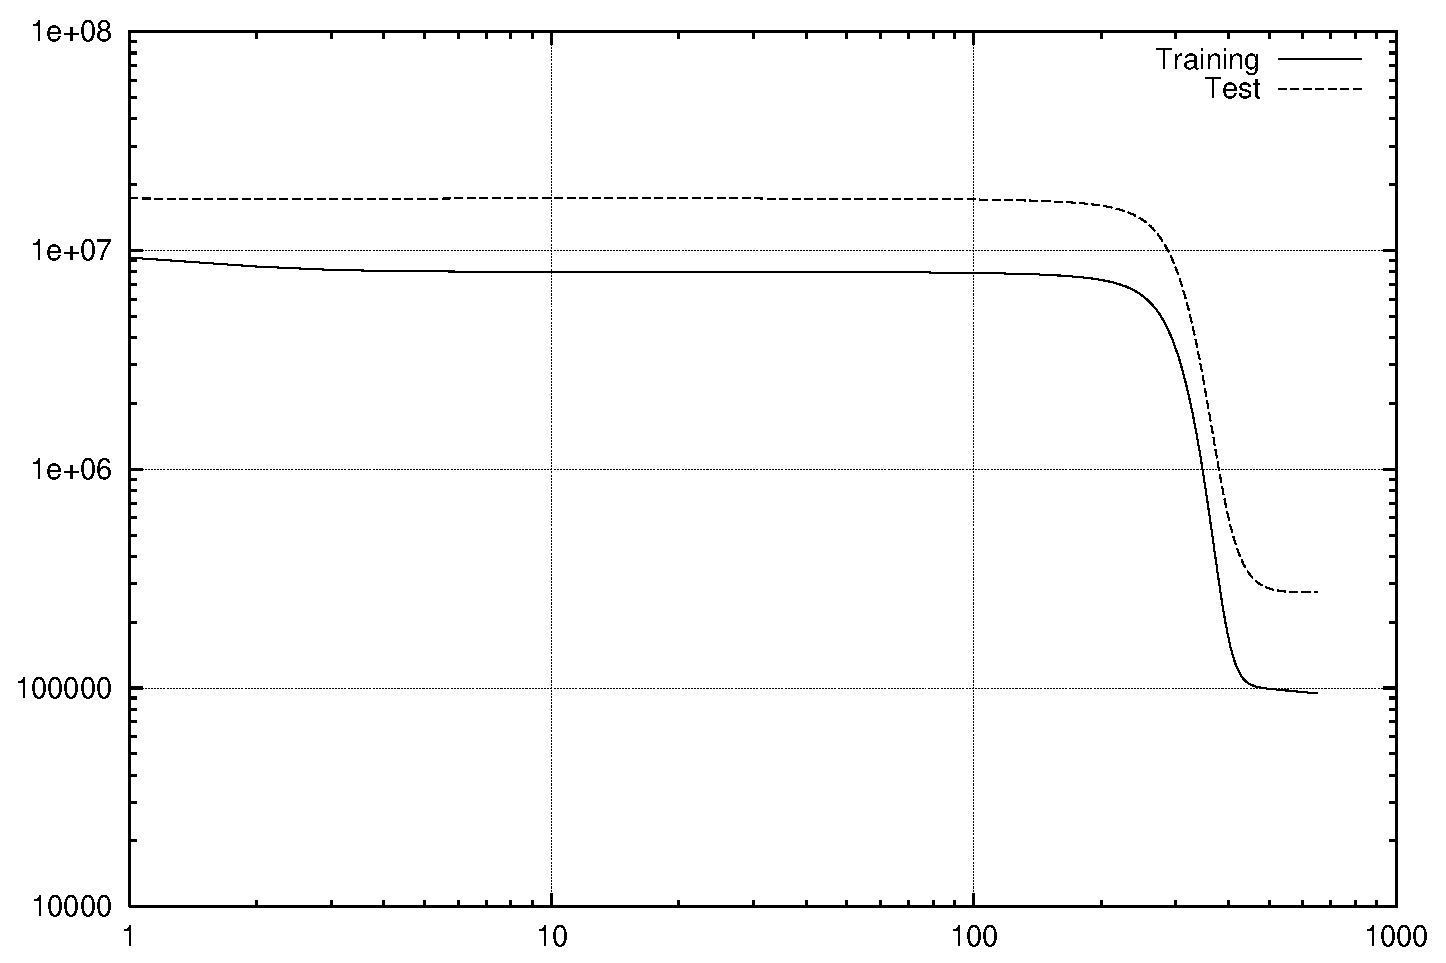
\includegraphics[width=0.8\textwidth,%
                     totalheight=0.35\textheight]{moby_nnc_pretr_training}\\
    & {\small Эпохи} \\
\end{tabular}
\caption{Ошибка имитации П-регулятора в процессе обучения НС--Р на
обучающей (сплошная линия) и тестовой (пунктирная линия) выборках.}
\label{fig:moby_nnc_pretr_training}
\end{figure}

\begin{figure}
\centering
\begin{tabular}{lclc}
  \begin{sideways}
    {\hspace{1cm}\small Управляющее воздействие}
  \end{sideways}
  &
  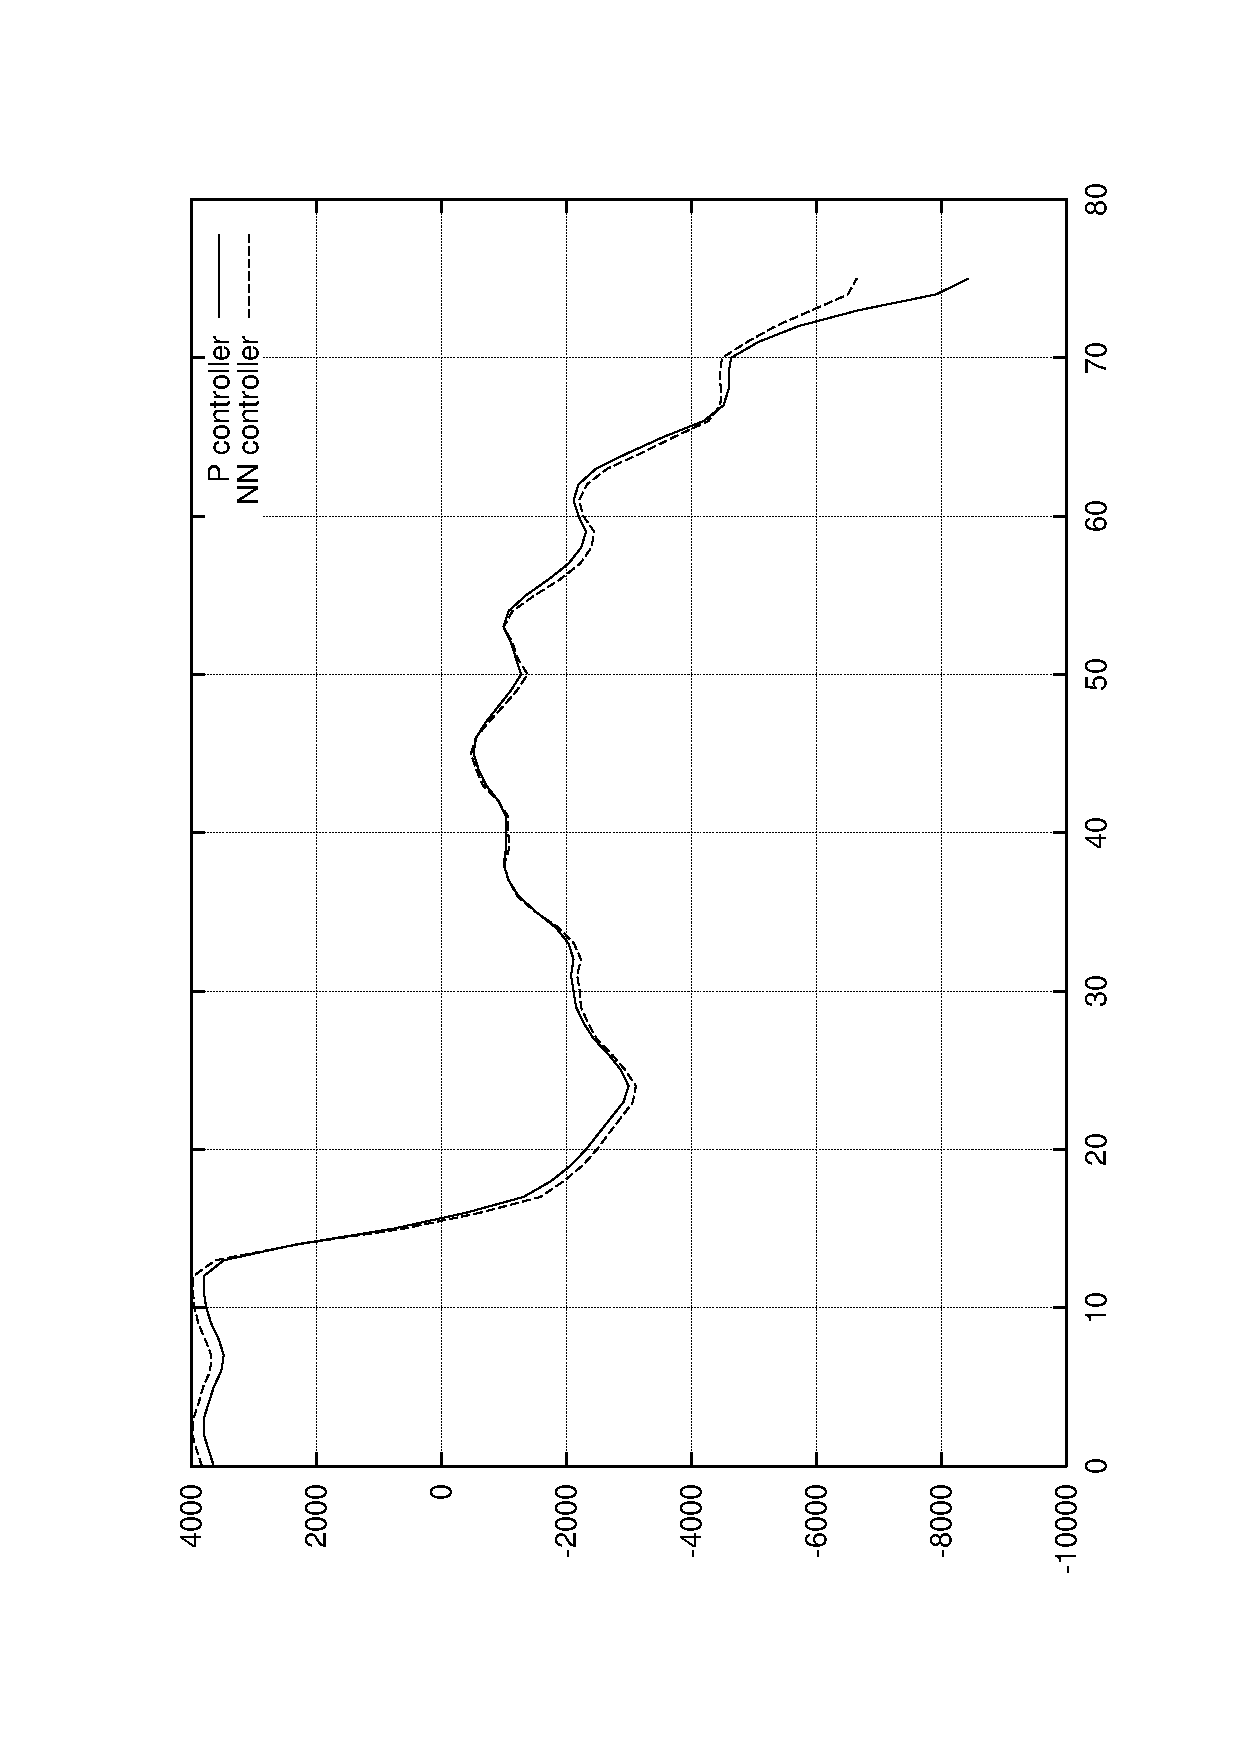
\includegraphics[width=0.45\textwidth,%
    totalheight=0.25\textheight]{moby_nnc_pretr_learn}
  &
  \begin{sideways}
    {\hspace{1cm}\small Управляющее воздействие}
  \end{sideways}
  &
  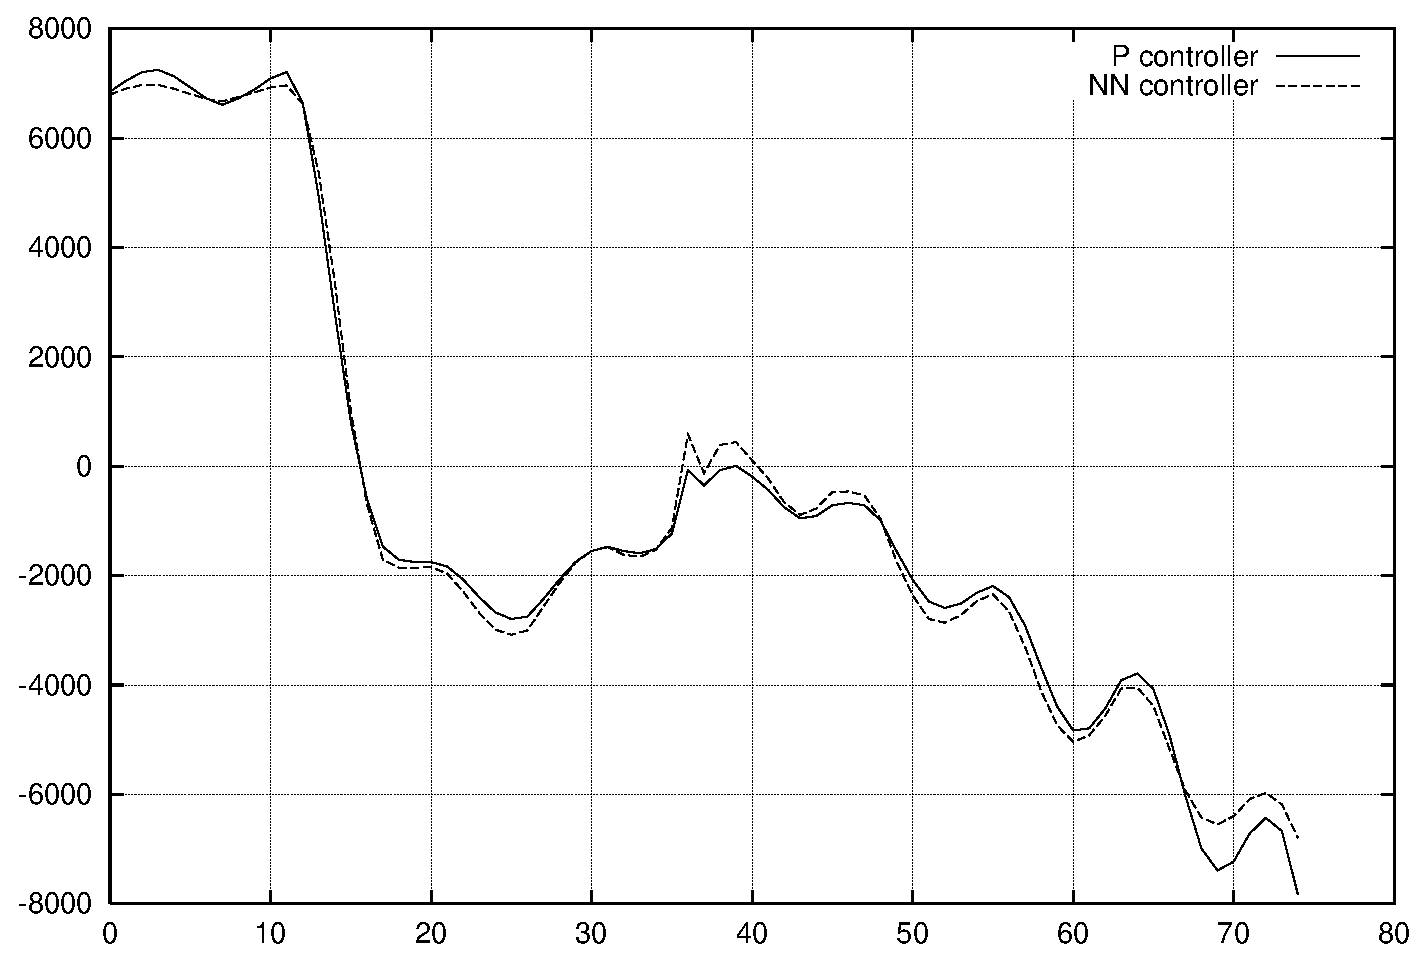
\includegraphics[width=0.45\textwidth,%
    totalheight=0.25\textheight]{moby_nnc_pretr_test}
  \\
  & {\small Время} & & {\small Время}\\
  & а) & & б)\\
\end{tabular}
\caption{Графики управляющего воздействия П-регулятора и их
имитация обученным нейросетевым регулятором.  Представлены траектории
из обучающей (а) и тестовой (б) выборок.  Сплошная линия ---
П-регулятор, пунктирная --- обученный НС--Р.}
\label{fig:moby_nnc_pretr}
\end{figure}

\subsection{Архитектура и обучение нейросетевой модели}

Учитывая нелинейность рассматриваемого объекта управления, для
нейросетевой модели предсказания была выбрана архитектура с одним
скрытым слоем с 5 нейронами и четырьмя входами
$\NN^o_{2+2,5,1}(u_k,u_{k-1},y_k,y_{k-1})$.  Входы
$u_k,u_{k-1},y_k,y_{k-1}$ обеспечивают сеть прямого распространения
информацией о динамике объекта.

Данные для обучения НС--О были получены в тех же десяти
экспериментальных заездах с П-регулятором в контуре, что и для
обучения НС--Р (см.~\figref{fig:moby_pc_x0-9_explore}).  Полученные
выборки ${u_k,y_k}$ были разделены на обучающие и тестовые.

\begin{figure}
\centering
  \begin{tabular}{rc}
    \begin{sideways}
      {\hspace{3cm}\small Координата маяка}
    \end{sideways}
    &
    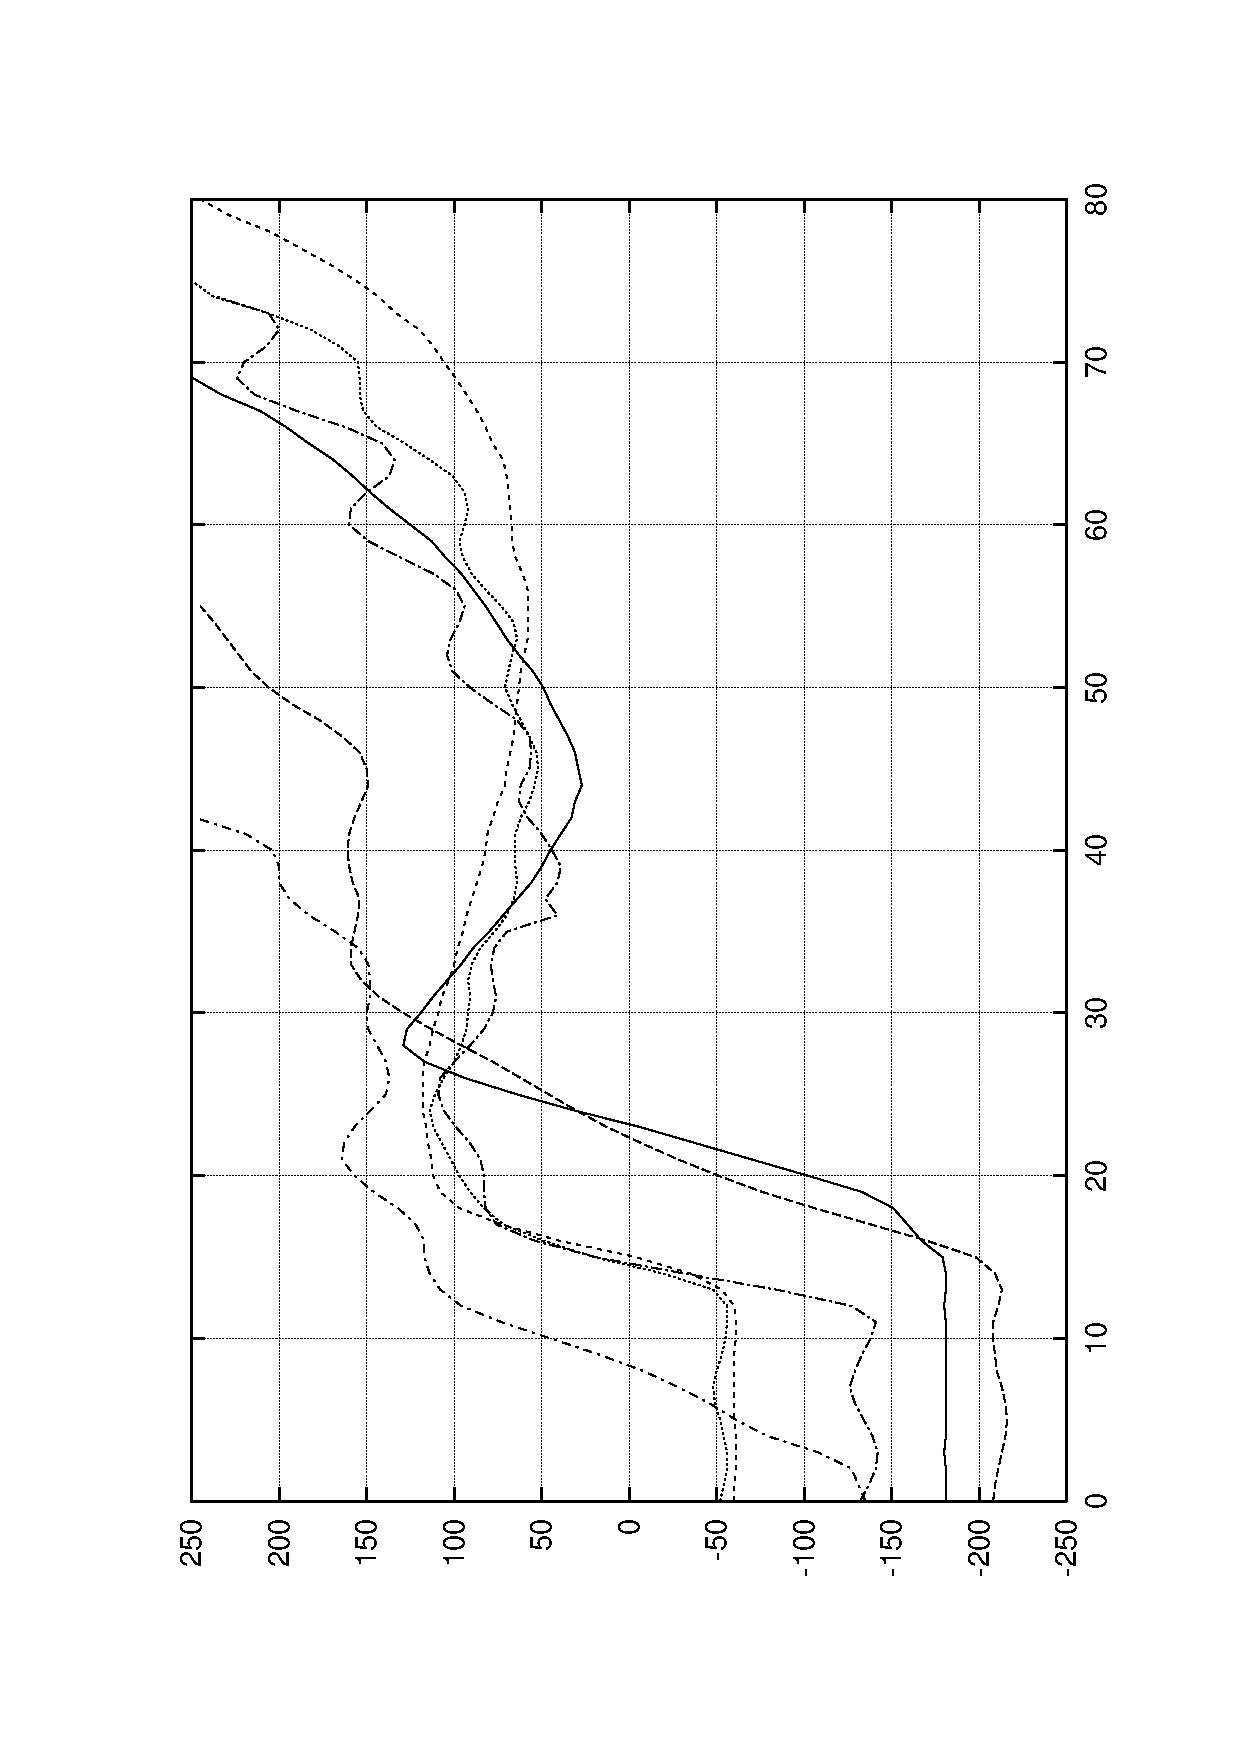
\includegraphics[width=0.8\textwidth,%
                     totalheight=0.35\textheight]{moby_pc_x0-9_explore}\\
    & {\small Время, отсчеты} \\
\end{tabular}
\caption{Траектории маяка в поле зрения видеокамеры робота в процессе 10
заездов с П-регулятором в контуре управления.}
\label{fig:moby_pc_x0-9_explore}
\end{figure}

Обучение нейросетевой модели проходило в пакетном режиме с
коэффициентом $\eta=0.03$ для скрытых слоев и $\eta=0.003$ для
выходного нейрона.  По истечении 435 эпох было обнаружено
систематическое увеличение ошибки предсказания выхода объекта на
тестовой выборке и процесс обучения НС--О был завершен.

Траектории среднеквадратической ошибки предсказания выхода объекта
нейросетевой моделью по обучающей и тестовой выборкам в процессе
пакетного обучения приведены на~\figref{fig:moby_nnp_training}.
Примеры траекторий, использовавшихся для обучения и результат
предсказания обученной нейросетевой моделью приведены
на~\figref{fig:moby_nnp}.

\begin{figure}
\centering
  \begin{tabular}{rc}
    \begin{sideways}
      {\hspace{4cm}\small Ошибка}
    \end{sideways}
    &
    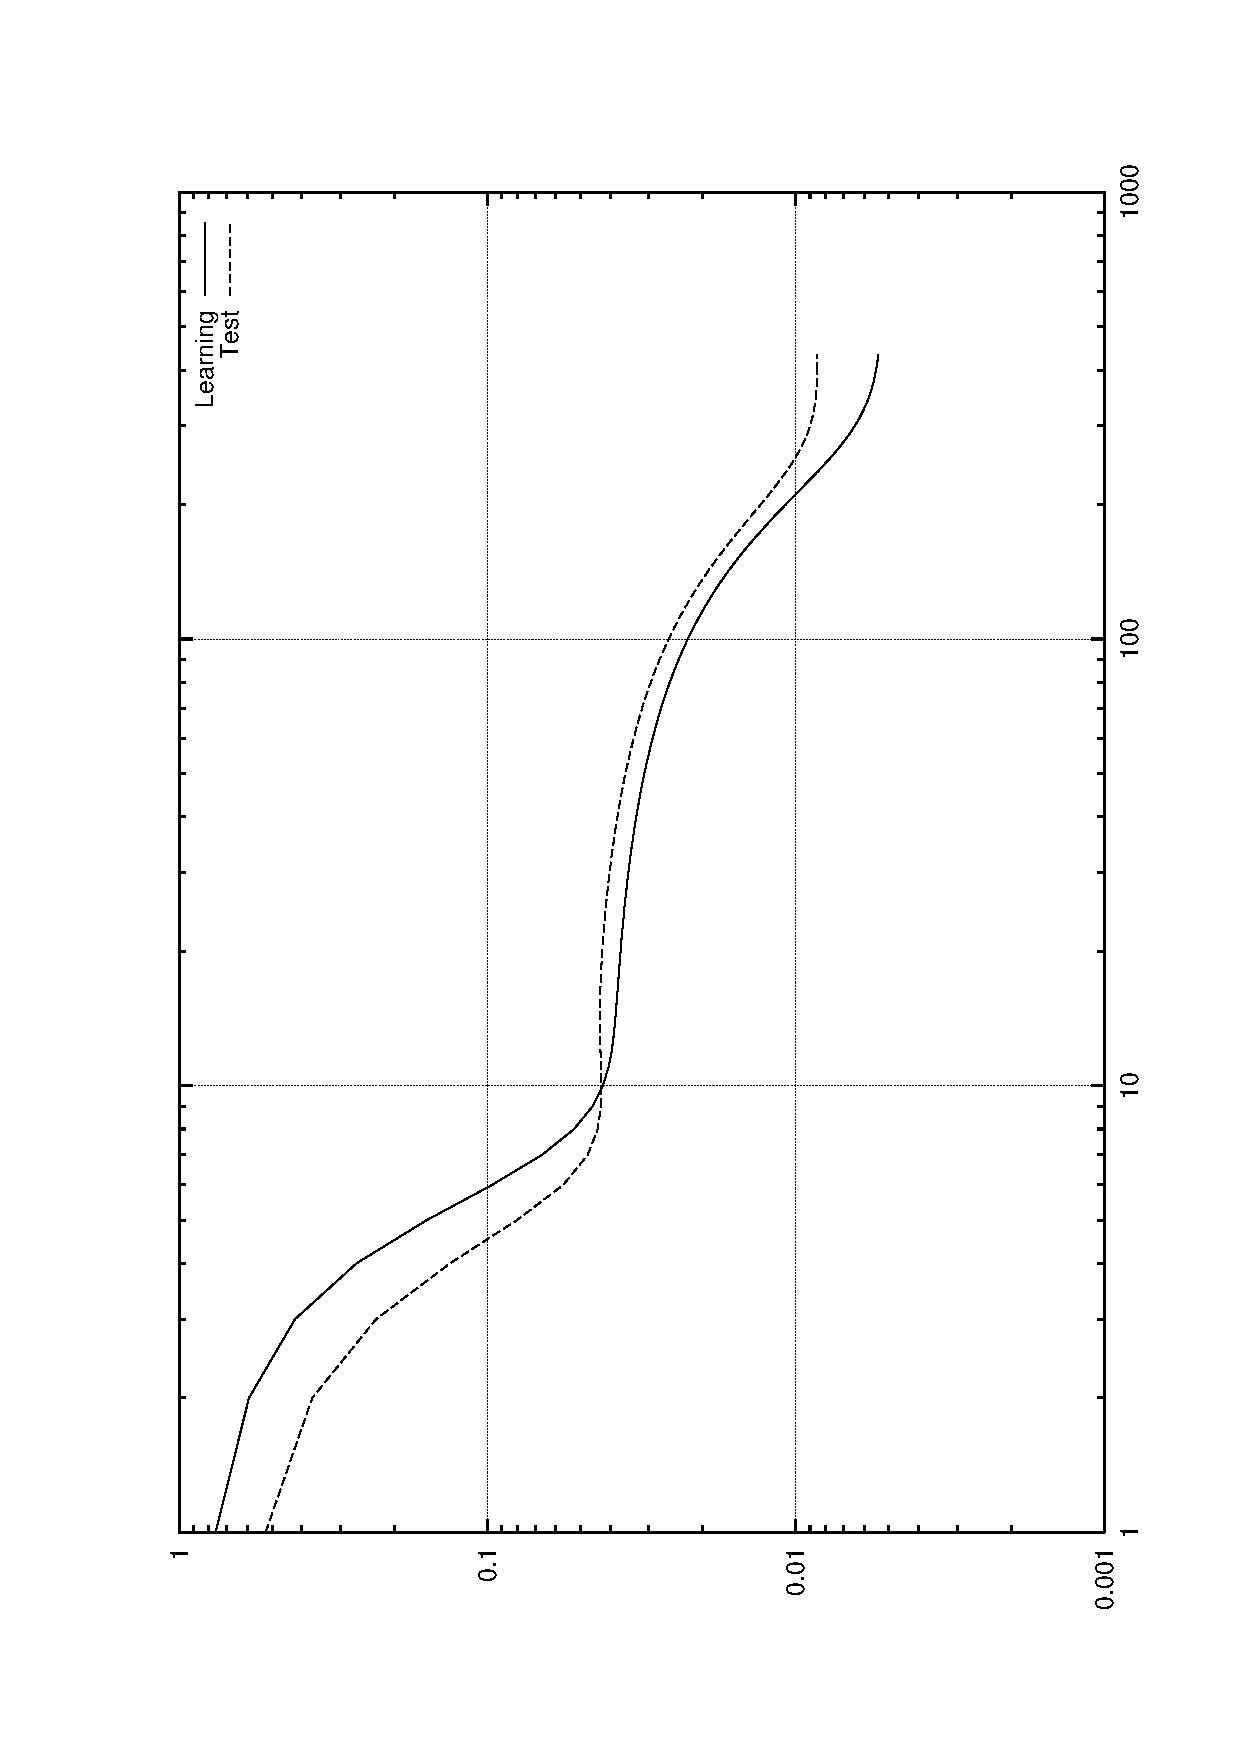
\includegraphics[width=0.8\textwidth,%
                     totalheight=0.35\textheight]{moby_nnp_training}\\
    & {\small Эпохи} \\
\end{tabular}
\caption{Ошибка предсказания нейросетевой модели объекта в процессе обучения
на обучающей (сплошная линия) и тестовой (пунктирная линия) выборках.}
\label{fig:moby_nnp_training}
\end{figure}

\begin{figure}
\centering
\begin{tabular}{lclc}
  \begin{sideways}
    {\hspace{1.7cm}\small Координата маяка}
  \end{sideways}
  &
  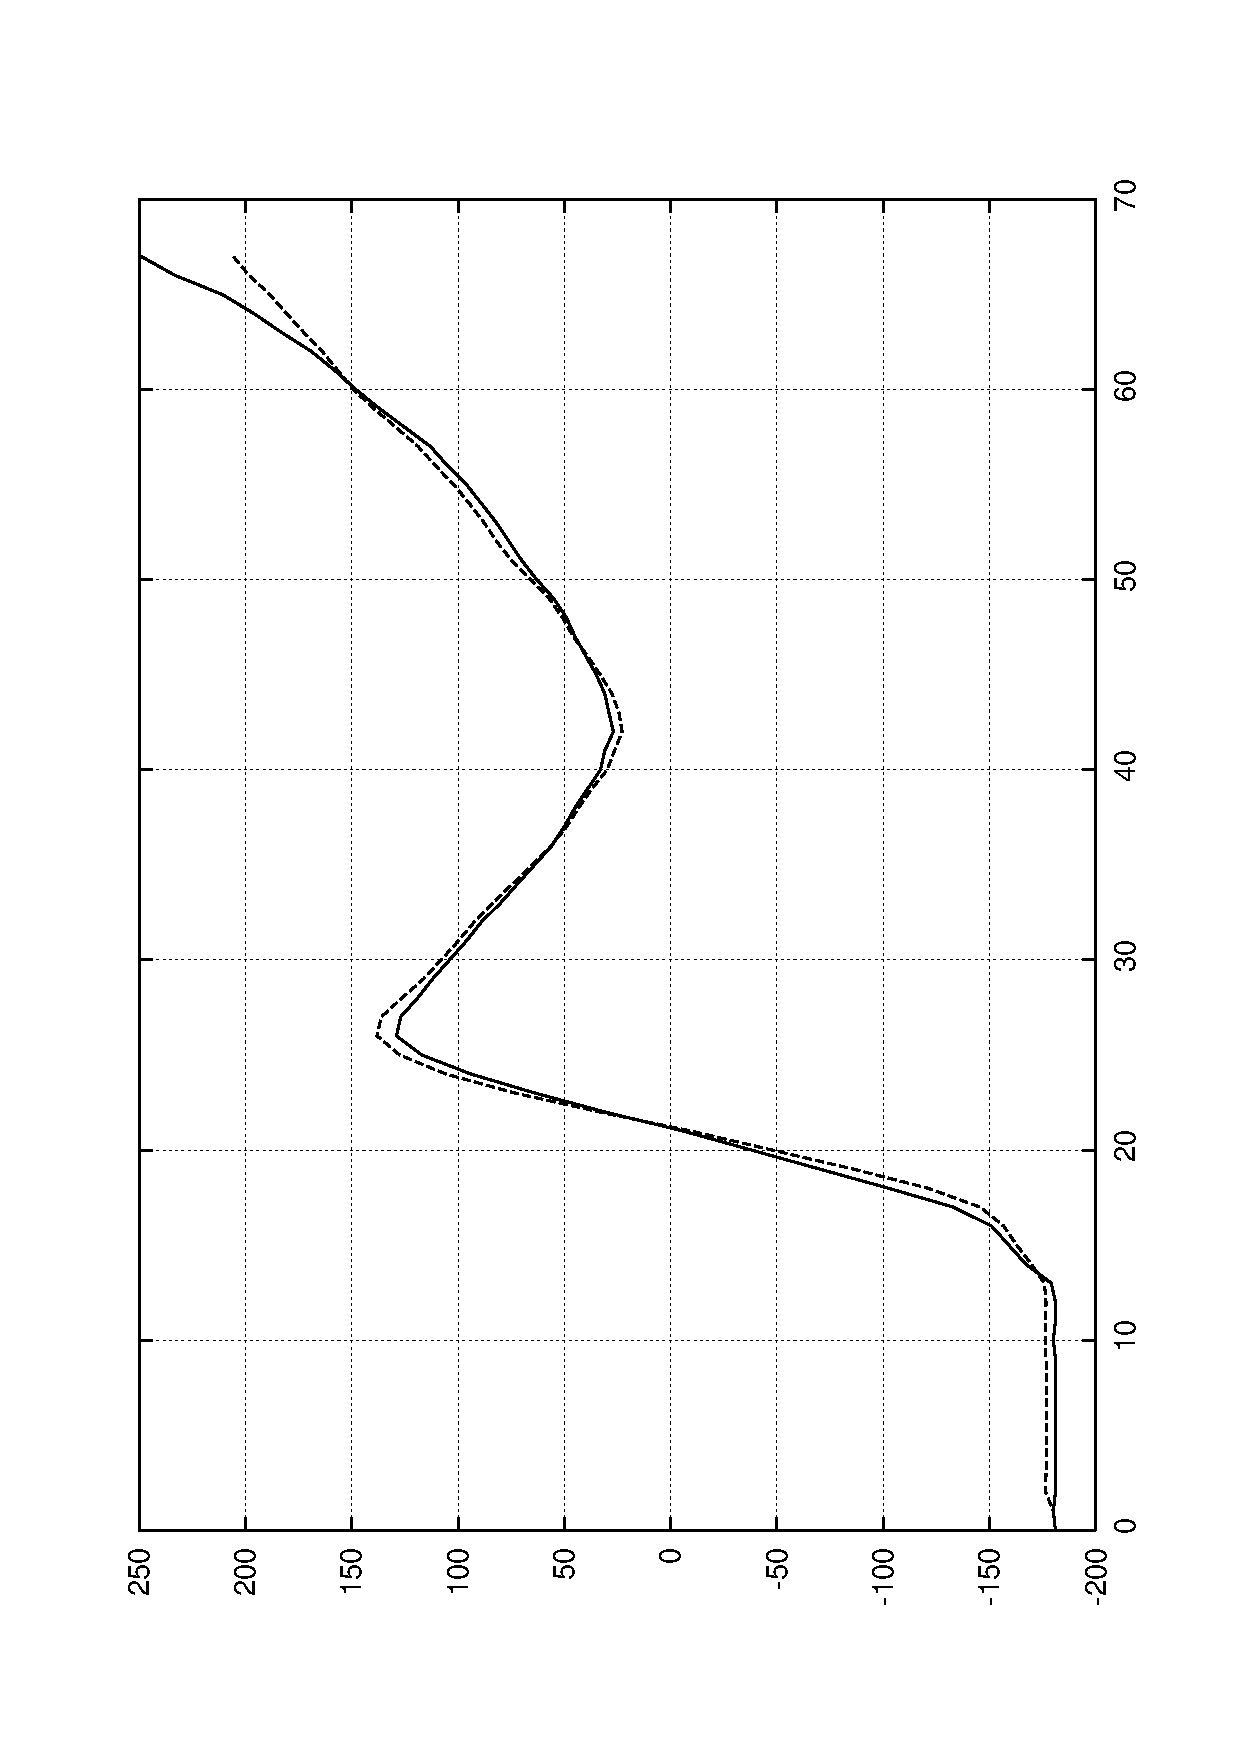
\includegraphics[width=0.45\textwidth,%
    totalheight=0.25\textheight]{moby_nnp_learn_no_title}
  &
  \begin{sideways}
    {\hspace{1.7cm}\small Координата маяка}
  \end{sideways}
  &
  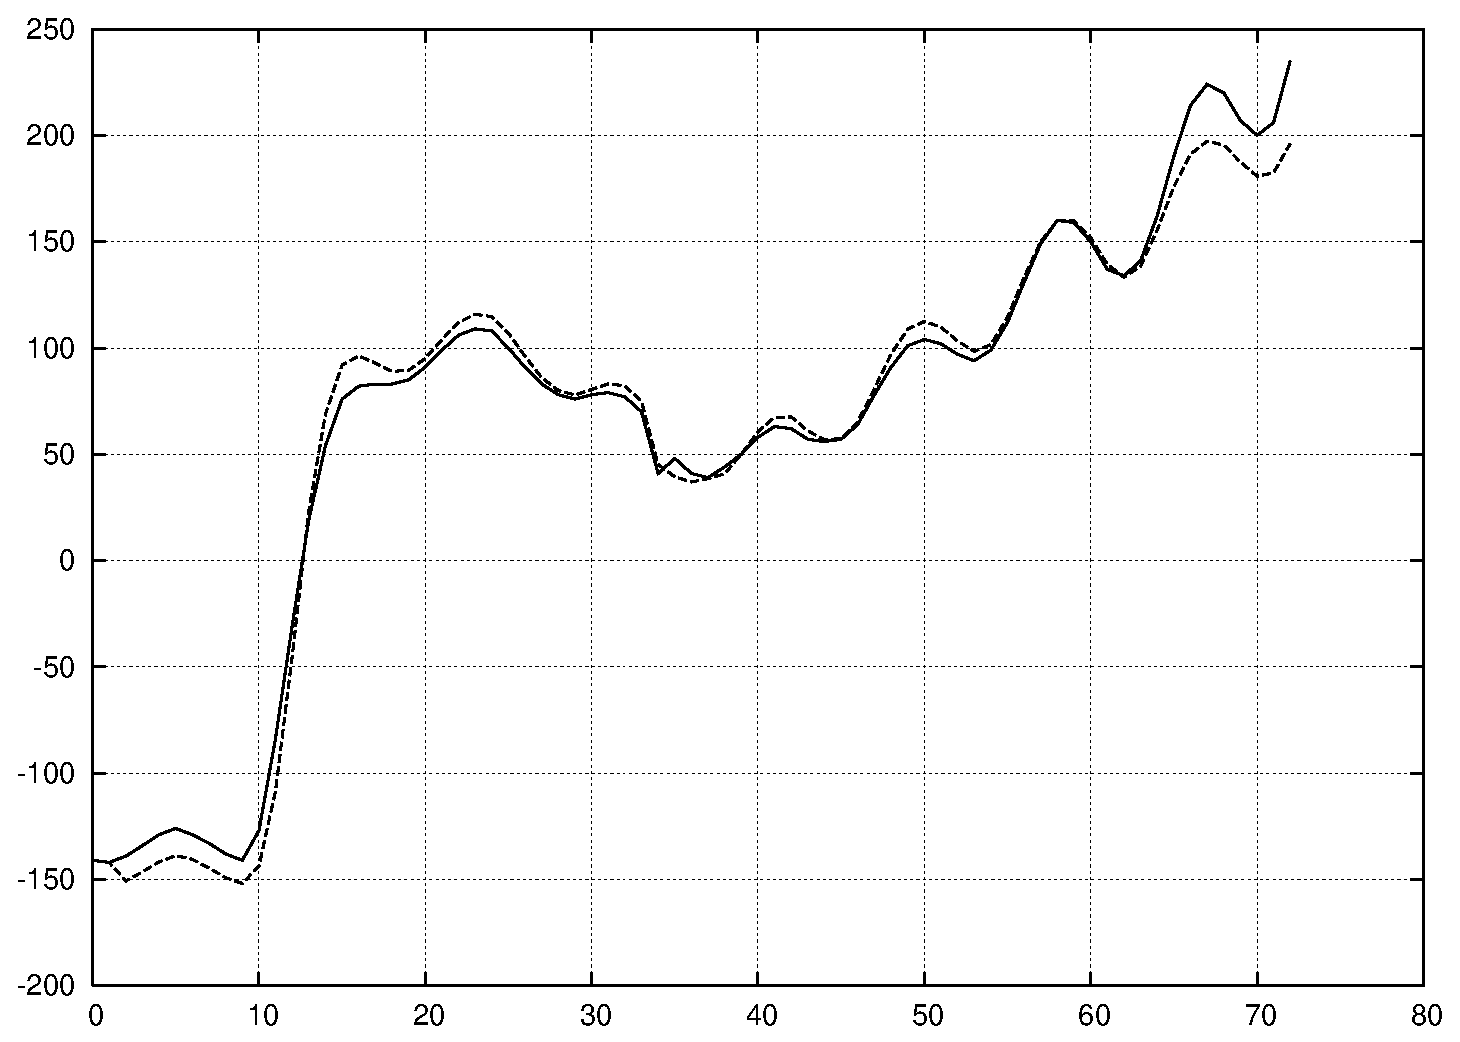
\includegraphics[width=0.45\textwidth,%
    totalheight=0.25\textheight]{moby_nnp_test_no_title}
  \\
  & {\small Время} & & {\small Время}\\
  & а) & & б)\\
\end{tabular}
\caption{Графики траектории маяка при управлении П-регулятором и их
предсказание обученной нейросетевой моделью.  Показаны траектории
из обучающей (а) и тестовой (б) выборок.  Сплошная линия --- выход объекта
управления, пунктирная --- предсказание обученной НС--О.}
\label{fig:moby_nnp}
\end{figure}

\subsection{Оптимизация нейросетевого регулятора}

Для оптимизации нейросетевого регулятора в контуре управления, то
есть, в процессе управления реальным роботом, были проведены
необходимые работы по адаптации программ моделирования и обучения
нейронных сетей к операционной среде компьютера, установленного на
мобильном роботе.  После этого в мобильный робот были загружены
нейронные сети регулятора и модели объекта, обученные вне контура.
Это дало возможность в процессе заездов при включенном алгоритме
обучения осуществлять подстройку весовых коэффициентов НС--Р с целью
минимизации ошибки по траектории.

В процессе заезда накапливались изменения весовых коэффициентов НС--Р,
которые применялись по его окончании.  Расчет поправок весовых
коэффициентов производился по методике, изложенной в
главе~\ref{neural_optimal_control} с инверсией объекта управления по
нейросетевой модели.  Коэффициенты скорости обучения для НС--Р были
взяты: для скрытых нейронов $\eta=0.05$, для выходного нейрона
$\eta=0.001$.

Было проведено всего 10 обучающих заездов.  Траектории координаты
маяка в процессе заездов продемонстрированы
на~\figref{fig:moby_nnc_x01-10_learn}.  Анализ траекторий показывает,
что постепенно нейросетевой регулятор изменяет свой поведение,
изначально имитирующее исходный П-регулятор
(ср.~\figref{fig:moby_pc_x0-9_explore}).  Характер траектории
усложняется, становится более осциллирующим.  При этом даже визуально
траектории становятся ближе к нулю.

\begin{figure}
\centering
  \begin{tabular}{rc}
    \begin{sideways}
      {\hspace{3cm}\small Координата маяка}
    \end{sideways}
    &
    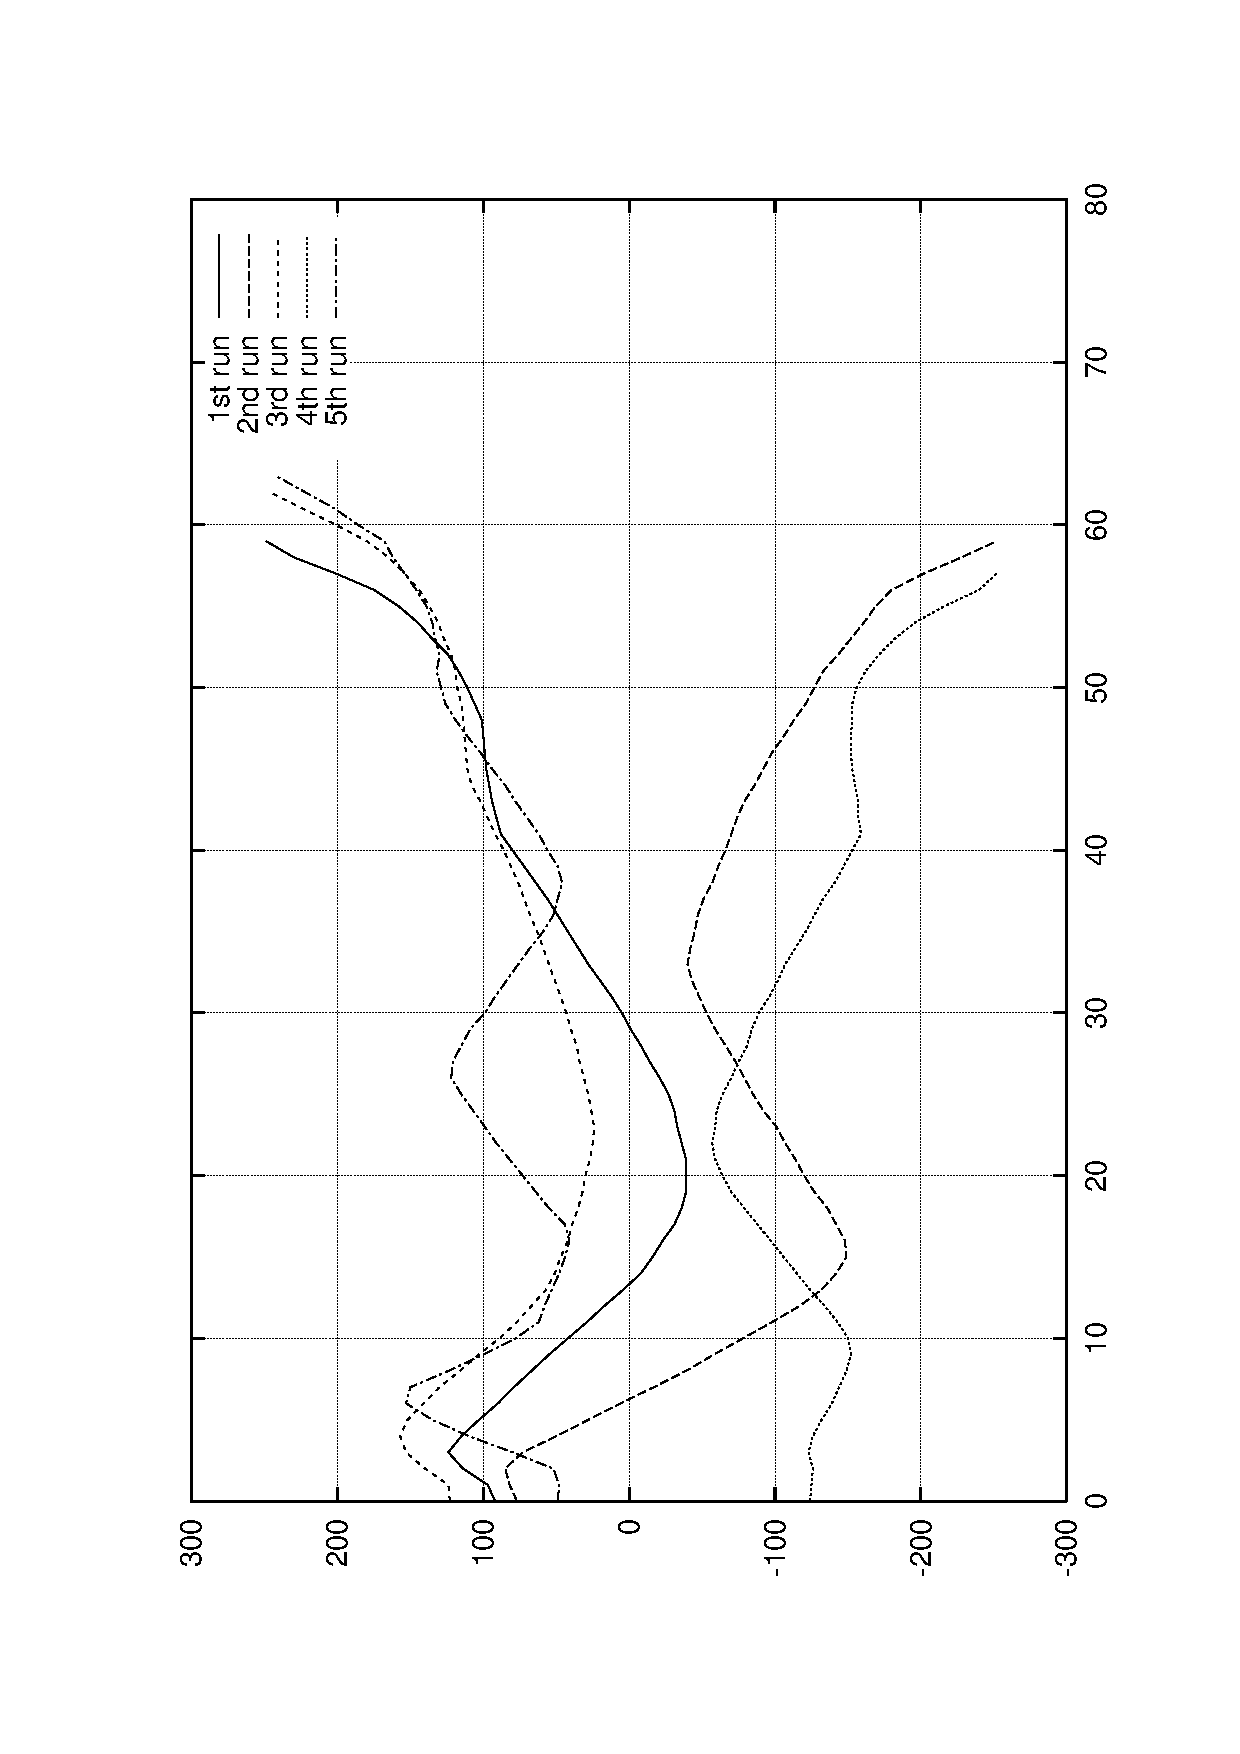
\includegraphics[width=0.8\textwidth,%
                     totalheight=0.35\textheight]{moby_nnc_x01-05_learn}\\
    & {\small Время, отсчеты} \\
    & а) \\
    \begin{sideways}
      {\hspace{3cm}\small Координата маяка}
    \end{sideways}
    &
    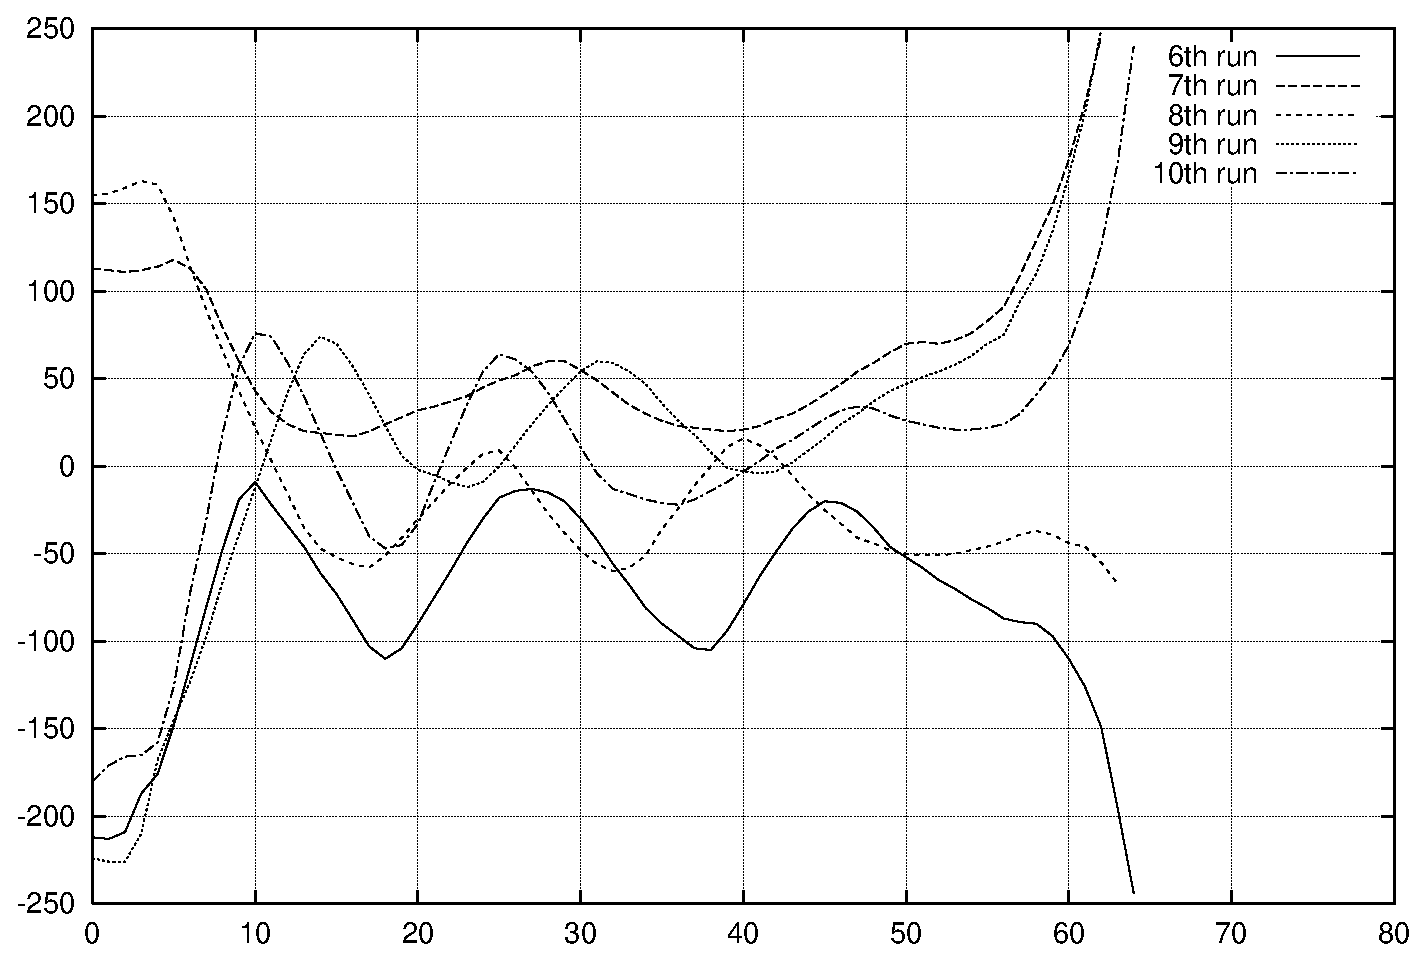
\includegraphics[width=0.8\textwidth,%
                     totalheight=0.35\textheight]{moby_nnc_x06-10_learn}\\
    & {\small Время, отсчеты} \\
    & б) \\
\end{tabular}
\caption{Траектории маяка в процессе 10 обучающих заездов, сгруппированные
поровну на первые (а) и последние (б).}
\label{fig:moby_nnc_x01-10_learn}
\end{figure}

По окончании обучения НС--О и алгоритм подстройки весовых
коэффициентов НС--Р были отключены.  Результаты тестовых заездов с
полученным нейросетевым оптимальным регулятором в контуре приведены
на~\figref{fig:moby_fnnc_x01-06_test}.

\begin{figure}
\centering
  \begin{tabular}{rc}
    \begin{sideways}
      {\hspace{3cm}\small Координата маяка}
    \end{sideways}
    &
    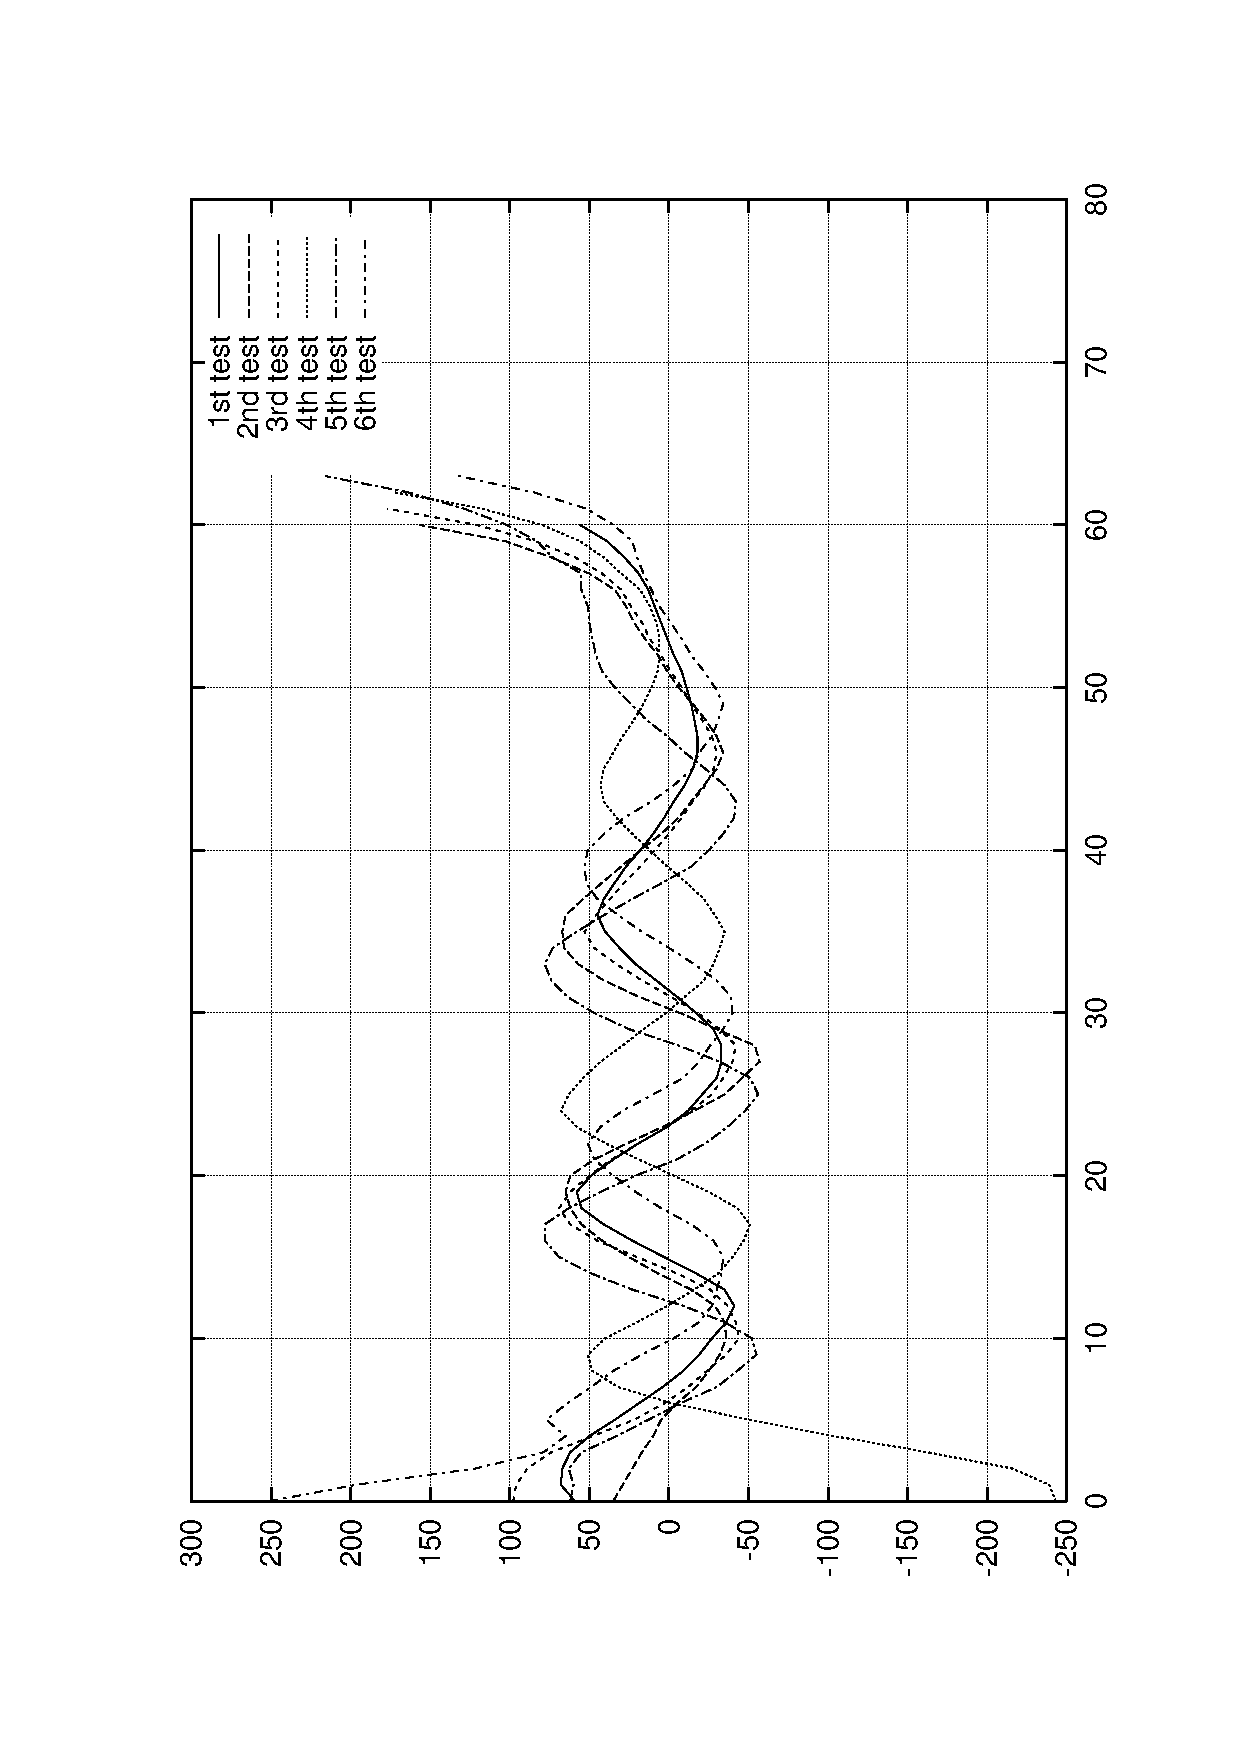
\includegraphics[width=0.8\textwidth,%
                     totalheight=0.35\textheight]{moby_fnnc_x01-06_test}\\
    & {\small Время, отсчеты} \\
\end{tabular}
\caption{Траектории маяка в поле зрения видеокамеры робота в процессе 6
тестовых заездов с обученным НОР в контуре управления.}
\label{fig:moby_fnnc_x01-06_test}
\end{figure}

\section{Сравнительный эксперимент}

По окнчании обучения нейросетевого оптимального регулятора был
осуществлен сравнительный эксперимент, позволяющий оценить достигнутые
результаты.  Было проведено 16 заездов с П-регулятором в контуре и 16
заездов с НОР (с отключенным алгоритмом обучения).

Качество управления оценивалось по минимальному достигнутому
расстоянию трактории мобильного робота до маяка.  Результаты заездов
приведены в~\tablref{tabl:moby_pc_noc_cmp}.  Из таблицы однозначно
следует вывод осущественном повышении качества управления при замене
П-регулятора на нейросетевой оптимальный.

\begin{table}
\caption{Величина промаха ($e$) мимо маяка (в мм).}\label{tabl:moby_pc_noc_cmp}
\begin{tabular}{|l|c|c|}
\hline
$\mathrm{N}^o$ & П-регулятор & НОР \\
\hline
1&	173&	58\\
2&	201&	47\\
3&	179&	22\\
4&	147&	57\\
5&	218&	29\\
6&	216&	72\\
7&	230&	39\\
8&	205&	40\\
9&	254&	44\\
0&	228&	79\\
11&	223&	79\\
12&	142&	40\\
13&	201&	77\\
14&	236&	53\\
15&	201&	29\\
16&	251&	29\\
\hline
$\bar e$       & 206.6&	49.6\\
$\bar\sigma^2_e$& 33.0 &	19.1\\
\hline
\end{tabular}
\end{table}

\subsection{Выводы}

% Конец Главы
